\documentclass[a4paper,12pt]{article}
\usepackage{amssymb} % needed for math
\usepackage{amsmath} % needed for math
\usepackage[utf8]{inputenc} % this is needed for german umlauts
\usepackage[ngerman]{babel} % this is needed for german umlauts
\usepackage[T1]{fontenc}    % this is needed for correct output of umlauts in pdf
\usepackage[margin=2.5cm]{geometry} %layout
\usepackage{booktabs}
\usepackage{hyperref}
\hypersetup{pdftitle={Balanced Banana},bookmarks=true,}
\usepackage{graphicx}
\usepackage{csquotes}
\usepackage[nonumberlist]{glossaries}
\usepackage{enumitem}
\usepackage{verbatim}
\usepackage{indentfirst} % Adds indent for the first paragraph after a {/section}


\deftranslation[to=ngerman]{Glossary}{\section{Stichwortverzeichnis}}

\makeatletter
\newenvironment{mycode}
 {\def\@xobeysp{\ }\verbatim\rightskip=0pt plus 6em\relax}
 {\endverbatim}
\makeatother

\setitemize{align=parleft, labelsep=0.5cm}


\makenoidxglossaries

\newglossaryentry{CLI}
{
	name=CLI,
	description={Befehlszeile, engl. Commandline Interface},
}

\newglossaryentry{CPU}
{
	name=CPU,
	description={Central Processing Unit, Kern jedes Rechners um Anwendungen auszuführen},
}

\newglossaryentry{Daemon}
{
	name=Daemon,
	description={Ein Dienst der auf Anfragen reagiert und antwortet},
}
\newglossaryentry{Client}
{
	name={Client},
	description={Programm auf dem Computer eines Benutzers um mit dem Server zu  kommunizieren}
}
\newglossaryentry{Configfile}
{
	name={Configfile},
	description={Eine Datei die bestimmte Einstellungen speichert}
}

\newglossaryentry{Server}
{
	name={Server},
	description={Programm auf dem Server, der die Benutzer (Außenwelt) mit den Arbeitern (Privates Netzwerk) verbindet}
}

\newglossaryentry{Benutzer}
{
	name={Benutzer},
	description={Eine Person, die dazu in der Lage ist, Befehle auszuführen}
}

\newglossaryentry{Prioritaet}
{
	name={Priorität},
	plural={Prioritäten},
	description={Ein diskretes Maß für Wichtigkeit bzw. Relevanz. Meist eine ganze Zahl, wobei gewisse Werte auch durch vorher definierte Wörter bezeichnet werden können}
}

\newglossaryentry{Multicast}
{
	name={Multicast},
	description={Eine Möglichkeit Nachrichten an mehrere Rechner gleichzeitig zu senden, ermöglicht eine Verbindungslose Kommunikation zwischen Client und Server. Auf einem vorher vereinbarten Kommunikationskanal (Es können mehrere Programme ungestört auf anderen Komunikationskanälen laufen).}
}

\newglossaryentry{Worker}
{
	name={Worker},
	description={Programm auf den Rechenknoten, welche dafür zuständig sind, die Aufgaben auszuführen}
}

\newglossaryentry{Administrator}
{
	name={Administrator},
	description={Eine Person, die dazu privilegiert ist, das Gesamtsystem zu verwalten und über uneingeschränkten Zugriff auf Ein- und Ausgabedateien verfügt}
}

\newglossaryentry{Task}
{
	name={Task},
	plural={Tasks},
	description={Jedes Programm (z.B. Skripte, Simulationen, etc.), das ein Benutzer auf einem Rechenknoten ausführen möchte}
}

\newglossaryentry{Rechenknoten}
{
	name={Rechenknoten},
	description={Leistungsstarke Rechner, die die von einem Benutzer gescheduelten Task ausführen}
}

\newglossaryentry{Statistik}
{
	name={Statistik},
	plural={Statistiken},
	description={Nützliche Informationen (z.B. Dauer der Task, Statuscode, etc.) über eine Task, die gesammelt werden sollen}
}

\newglossaryentry{Web-API}
{
	name={Web-API},
	description={Web-API (Web-Application Programming Interface) ist eine Art Schnittstelle über das Web, die über eine Reihe von Funktionen verfügt, die es Benutzern ermöglichen, auf bestimmte Funktionen oder Daten einer Applikation, eines Betriebssystems oder anderer Dienste zuzugreifen}
}

\newglossaryentry{Ausnahmebehandlung}
{
	name={Ausnahmebehandlung},
	description={Der Prozess der Reaktion auf das Auftreten von Ausnahmen  - außergewöhnliche Bedingungen, die eine spezielle Verarbeitung erfordern - während der Berechnung , die oft den normalen Ablauf der Programmausführung unterbrechen}
}

\newglossaryentry{Estimated Time of Arrival}
{
	name={ETA},
	description={Der Zeitpunkt, zu dem eine Task erledigt wird}
}

\newglossaryentry{Concurrency}
{
	name={Concurrency},
	description={Die Eigenschaft eines Systems, mehrere Berechnungen, Anweisungen oder Befehle gleichzeitig auszuführen}
}

\title{Balanced Banana}
\author{Niklas Lorenz \and Thomas Häuselmann \and Rakan Zeid Al Masri \and Christopher Lukas Homberger \and Jonas Seiler}


%%%%%%%%%%%%%%%%%%%%%%%%%%%%%%%%%%%%%%%%%%%%%%%%%%%%%%%%%%%%%%%%%%%%%%
% Create a shorter version for tables. DO NOT CHANGE               	 %
%%%%%%%%%%%%%%%%%%%%%%%%%%%%%%%%%%%%%%%%%%%%%%%%%%%%%%%%%%%%%%%%%%%%%%
\newcommand\addrow[2]{#1 &#2\\ }

\newcommand\addheading[2]{#1 &#2\\ \hline}
\newcommand\tabularhead{\begin{tabular}{lp{13cm}}
\hline
	}

\newcommand\addmulrow[2]{ \begin{minipage}[t][][t]{2.5cm}#1\end{minipage}%
   &\begin{minipage}[t][][t]{8cm}
    \begin{enumerate} #2   \end{enumerate}
    \end{minipage}\\ }

\newenvironment{usecase}{\tabularhead}
{\hline\end{tabular}}

\usepackage{microtype}

\begin{document}
\pagenumbering{roman}
\begin{titlepage}
    \begin{center}
    
     \vspace*{0.8cm}
 
        
\includegraphics[width=0.5\textwidth]{balancedbanana}
        \vspace*{1cm}
 
        \Huge
        \textbf{Balanced Banana}
 
        \vspace{0.5cm}
        \LARGE
        A Distributed Task Scheduling System
        
        \vspace{0.5 cm}
        \LARGE
        Pflichtenheft
 
        \vspace{1.5cm}

        \large
        \textbf{Niklas Lorenz, Thomas Häuselmann, Rakan Zeid Al Masri, Christopher Lukas Homberger und Jonas Seiler}
 
        \vspace*{0.5cm}

        \textbf{\today}
 
       
        
 
    \end{center}
\end{titlepage}         % Deckblatt.tex laden und einfügen
\setcounter{page}{2}
\tableofcontents          % Inhaltsverzeichnis ausgeben
\clearpage
\pagenumbering{arabic}

\section{Einleitung}
\vspace*{1cm}

Die Verteilung rechenintensiver Aufgaben ist ein in vielen Unternehmen übliches Problem. Wenn ein Team größer wird, 
so werden auch die verfügbaren Rechenressourcen und die darauf ausgeführten Aufgaben größer und komplexer sein.\\


Es wird immer schwieriger, die vorhandenen Ressourcen effizient und gerecht auf die verschiedenen Mitarbeiter und Aufgaben aufzuteilen.
Aktuell stehen nur einzelne Rechner zur Verfügung, die von jedem Mitarbeiter beliebig verwendet werden können. So können Aufgaben nur bearbeitet werden,
wenn zum Zeitpunkt der Anfrage ein Rechner frei steht. Doch das ist weder fair den einzelnen Nutzern gegenüber, noch kann die Hardware dadurch gut ausgelastet werden. Wird eine Aufgabe beispielsweise mitten in der Nacht abgeschlossen, ist niemand da, um eine neue Aufgabe ausführen zu lassen. \\


Es gibt auf dem Markt bereits viele Lösungen für dieses Problem, allerdings sind sie sehr komplex und nicht leicht erweiterbar.
Balanced Banana soll dieses Problemes in Form eines kompakten, einfach zu bedienenden und skalierbaren Programms lösen. \\

Mit unserem Programm soll der Benutzer seine Aufgaben einfach von der Kommandozeile absetzen können, die dann automatisch auf die bereitstehende Hardware verteilt werden. \\

Darüber hinaus soll der Benutzer durch die Verwendung von zusätzlichen Parametern in der Lage sein, weitere Einschränkungen und/oder Bedingungen für seine Aufgaben anzugeben.\\

Mit Hilfe intelligenter Algorithmen soll unser Programm in der Lage sein die verfügbaren Rechenressourcen für die anstehenden Aufgaben effizient zu verteilen,
basierend auf Größe, Priorität und gegebenen Einschränkungen und Bedingungen. Um möglichst flexibel einsetzbar zu sein, soll außerdem die Verteilalgorithmik
über eine feste Schnittstelle jederzeit änderbar sein, sodass Aspekten wie Fairness oder Turnaround-Zeit unterschiedliche Priorität eingeräumt werden kann.

\clearpage
\section{Zielbestimmung}
\subsection{Musskriterien}
\begin{itemize}[nosep]
	
	\item Der Benutzer kann seine Aufgabe einfach von der Kommandozeile absetzen.
	
	\item Parameter ermöglichen die Angabe weiterer Optionen, zum Beispiel das Setzen einer Priorität oder Anforderungen für die Tasks. 
		
	\item Balanced Banana soll in der Lage sein, die Tasks des Benutzers auf die \gls{Rechenknoten} zu verteilen.
	
	\item Balanced Banana soll das oben genannte Ziel mit minimalem Aufwand für den Benutzer erfüllen.
	
	\item Vom Benutzer gescheduelte \glspl{Task} sollen nicht manuell gestartet werden müssen. Balanced Banana macht dies automatisch.
	
	\item Balanced Banana sammelt \glspl{Statistik} über \glspl{Task} und stellt sie den Benutzern zur Verfügung.
	
	\item Die Anzahl der Worker ist leicht anpassbar.
	
	\item Der Benutzer ist in der Lage, verschiedene Prioritäten für Tasks zu setzen.
	
	\item Der Benutzer soll benachrichtigt werden, wenn eine Task erledigt ist oder fehlschlägt.
	
	\item Statistiken sollen über eine \gls{Web-API} mit HTTP-Requests bereitgestellt werden.
	
	\item Die \gls{Web-API} ermöglicht eine einfache Integration der Balanced Banana-Statistik in andere Projekte (z.B. das SmartTV-Projekt).
	
	\item Das Programm ist ausführlich dokumentiert und enthält klare Anleitungen zur Benutzung.

\end{itemize}

\subsection{Wunschkriterien}
\begin{itemize}[nosep]

	\item Der Benutzer kann \glspl{Task} pausieren.	
	
	\item Das Programm kann die \gls{Estimated Time of Arrival} für die verbleibenden Tasks vorhersagen.
	
	\item Mehrsprachige Benachrichtigung.
	
	\item Andere Benutzer können den Status anderer Tasks verfolgen und sich darüber benachrichtigen lassen.
	
	\item Der Benutzer kann die Ausführung einer Task verzögern (z.B. wenn eine Task in 30 Minuten ausgeführt werden soll).
	
\end{itemize}

\subsection{Abgrenzungskriterien}
\begin{itemize}[nosep]

	\item Das Programm führt die gescheduelten \glspl{Task} nicht persönlich aus, sondern überlässt die Arbeit den \gls{Rechenknoten}.
	
	\item Das Programm macht nichts mit der Ausgabe der verschiedenen Tasks, es verteilt nur die Tasks.
	
	\item Das Programm macht keine \gls{Ausnahmebehandlung}. Es geht davon aus, dass die an es gesendeten Tasks fehlerfrei funktionieren.
	
	\item Das Programm macht nichts mit den gesammelten \glspl{Statistik}, es lässt den Benutzer sie nur über die \gls{Web-API} sehen.
	
	\item Das Programm ermöglicht keine \gls{Concurrency} von Tasks auf einem Rechenknoten.
	
\end{itemize}

% Was will ich bewusst nicht umsetzen?
% Was soll es nicht sein?

% Ist das nicht ne Wiederholung von Einleitung + Anforderungen?
% Ich würde das sehr kurz halten, so wie die Einleitung zum Beispiel

\clearpage
\section{Szenarien}

\subsection{\textbf{Einreihen einer Aufgabe in Warteschlange}}
Tom möchte eine Katzensimulation auf dem Rechenkluster simulieren lassen. %Alternative für Rechenkluster
Tom startet auf seinem PC den BalancedBanana-Client. Dieser verbindet sich im Hintergrund mit dem Hauptserver des Rechenklusters und authentifiziert Tom.
Nun reiht Tom seine Simulation auf der Kommandozeile mit normaler Priorität ein.
Tom sieht, dass alle Server ausgelastet sind und das er an zweiter Stelle in der Warteschlange steht.
Nach zwei Stunden sieht Tom erneut nach und stellt fest, dass er nun an vorderer Stelle in der Warteschlange steht.
Nach drei weiteren Stunden sieht er, dass seine Aufgabe aus der Warteschlange verschwunden ist und er eine E-mail erhalten hat.
In dieser steht, dass seine Aufgabe in 43 Minuten abgeschlossen wurde er erhält einen Link mit dem er die Ausgabe seiner Aufgabe einsehen kann.

\subsection{\textbf{Aufwerten der Priorität}}
Peter möchte eine wichtige Bauteilsimulation rechnen lassen.
Dazu startet Peter den BalancedBanana-Client und reiht seine Aufgabe mit normaler Priorität ein.
Nachdem Peter nach 3 Stunden keine Rückmeldung bekommen hat, prüft er die Warteschlange und sieht das Tom ein Duzent Katzensimulationen mit hoher Priorität eingereiht hat.
Genervt beendet Peter seinen PC und hofft das seine Simulation bis morgen abgeschlossen ist.
Am nächsten morgen bemerkt Peter das Tom ein weiteres Duzent Katzensimulationen mit erneut hoher Priorität eingereiht hat.
24 Stunden nach Einreihung seiner Aufgabe wird nun die Priorität dieser automatisch erhöht und hat nun ebenfalls hohe Priorität.
Peter bemerkt das seine Aufgabe nun in der Warteschlange langsam nach vorne rückt und schließlich gestartet wird. 
Nach einiger Zeit erhält Peter eine Email mit dem Ergebnis seiner Simulation.

\clearpage
\section{Produkteinsatz}
% Zielgruppe
% Anwendungsbereiche
% Betriebsbedinugen
% Wer? Was? Wozu?
\begin{itemize}
\begin{minipage}[t]{\linewidth}
\item \textbf{Zielgruppe}\newline
Das Produkt ist für die Verwendung durch die Mitarbeiter am Institut für Technische Informatik (ITEC) des Karlsruher Institut für Technologie (KIT) gedacht.\newline
Den Mitarbeitern soll die Benutzung der Arbeiter Rechner erleichtert werden, indem die Verteilung der Aufgaben automatisch erfolgt. Somit soll garantiert werden, dass die Aufgaben sich gegenseitig möglichst wenig stören.\newline
Durch die Vermeidung von Situationen, in denen mehrere Personen Aufgaben auf dem selben Rechner ausführen, während einer oder mehrere andere Arbeiter unbeschäftigt sind, soll die Leistungsfähigkeit sowie allgemeine Zufriedenheit und Harmonie gesteigert werden.
\end{minipage}
\\

\begin{minipage}[t]{\linewidth}
\item \textbf{Verwendungszweck}\newline
Das Produkt dient dazu, Simulationen und andere rechenintensive Aufgaben auf eigens zu diesem Zweck gedachte Rechner (Arbeiter) zu verteilen.\newline
Oftmals fallen Aufgaben an, die von einem Computer berechnet werden können und sollen. Nicht immer ist der eigene Rechner jedoch dieser Aufgabe gewachsen. Damit sich Benutzer und Aufgabe also nicht um Rechenzeit streiten, werden die anstehenden Aufgaben auf einen Pool von Arbeiter Rechnern verteilt, die speziell für diesen Zweck zur Verfügung stehen. Die Aufgabe des Verteilens wird von dem Produkt übernommen.
\end{minipage}
\\

\begin{minipage}[t]{\linewidth}
\item \textbf{Produktaufbau}\newline
Das Produkt ist den Aufgabengebieten entsprechend in drei Programme aufgeteilt:\newline
1. Der Client (Benutzer): Verantwortlich für die Interaktion des Benutzers mit dem Produkt auf der Befehlszeile.\newline
2. Der Scheduler (Server): Verantwortlich für das effiziente Verteilen der Aufgaben auf dem Arbeiterpool. Agiert als Mittelmann zwischen Benutzer und Arbeiter.\newline
3. Der Arbeiter (Worker): Verantwortlich für Ausführung, Pausieren und Abbruch der Aufgaben auf den Arbeitern (spezielle Rechner für die Aufgabenverarbeitung).
\end{minipage}
\end{itemize}
\newpage

\newpage
\section{Produktumgebung}
% Unter welcher Software / Hardware läuft es?

\begin{itemize}
\begin{minipage}[t]{\linewidth}
\item \textbf{Client (Nutzer) Umgebung}\newline
Das Benutzer Produkt ist für den Einsatz auf einem Rechner bestimmt, der folgenden Anforderungen genügt:
\subitem \textbf{Betriebssystem:} Linux oder ein Linux basiertes Betriebssystem
\subitem \textbf{CPU:} Mindestens ein CPU Kern
\subitem \textbf{Arbeitsspeicher:} Mindestens 1 GB verfügbarer Arbeitsspeicher
\end{minipage}
\\

\begin{minipage}[t]{\linewidth}
\item \textbf{Scheduler (Server) Umgebung}\newline
Das Server Produkt ist für den Einsatz auf einem Rechner bestimmt, der das Benutzer Netzwerk mit dem Arbeiter Netzwerk verbindet und folgenden Anforderungen genügt:
\subitem \textbf{Betriebssystem:} CentOS 7 oder Ubuntu 18.04
\subitem \textbf{CPU:} Mindestens ein CPU Kern
\subitem \textbf{Arbeitsspeicher:} Mindestens 4 GB verfügbarer Arbeitsspeicher
\end{minipage}
\\

\begin{minipage}[t]{\linewidth}
\item \textbf{Arbeiter (Worker) Umgebung}\newline
Das Arbeiter Produkt ist für den Einsatz auf einem Rechner bestimmt, der folgenden Anforderungen genügt:
\subitem \textbf{Betriebssystem:} CentOS 7 oder Ubuntu 18.04
\subitem \textbf{CPU:} Mindestens ein CPU Kern, Empfohlen: 24 CPU Kerne
\subitem \textbf{Arbeitsspeicher:} Mindestens 8 GB verfügbarer Arbeitsspeicher, Empfohlen: 64 GB Arbeitsspeicher
\end{minipage}
\end{itemize}
\newpage

\section{Funktionale Anforderungen}

\subsection{Übersicht der  Funktionalen Anforderungen}

 %Name ändern pls

\begin{itemize}[nosep]
\leftskip=0.5cm

\item[FA1]	\gls{Client} verbindet sich beim Starten mit dem Server.
\item[FA2] Benutzer authentifiziert sich über den \gls{Client} gegenüber dem Server.
\item[FA3] Benutzer kann eine Aufgabe in über \gls{Client} einreihen.
\item[FA4] Benutzer kann Parameter übergeben.
\item[FA41]	\gls{Client} speichert voreingestellte Parameter in \gls{Configfile}.
\item[FA42]	Benutzer kann Parameter über \gls{Configfile} übergeben.
\item[FA43] Benutzer kann \gls{Prioritaet} einer Aufgabe festlegen.
\item[FA44] Benutzer kann minimale und maximale Anzahl genutzer Kerne festlegen. %Glossar Kerne
 \item[FA45] Benutzer kann maximal nutzbaren RAM festlegen. %Glossar RAM
\item[FA46] Benutzer kann das benutzte Betriebssystem festlegen.
\item[FA47] Benutzer kann angeben ob der \gls{Client} blockieren soll bis die Aufgabe beendet ist. %Blockierbar glosar?
\item[FA48] Benutzer übergibt Pfad zu den für die Aufgabe benötigten Dateien. %Pfad glosar?
\item[FA49] Falls der Benutzer keine Parameter übergibt werden Standartwerte benutzt.
\item[FA5] Benutzer kann den Status einer Aufgabe einsehen.
\item[FA6] Benutzer bekommt Benachrichtigung über erledigte Aufgabe.
\item[FA7] Server erstellt regelmäßige Sicherungen von laufenden Aufgaben.
\item[FA8] Benutzer kann die Ausgabe seiner Aufgabe anfordern.
\end{itemize}

\subsection{Erläuterung der funktionalen Anforderungen}

\begin{comment}

%Format einer funktionalen Anforderung:
\begin{minipage}[t]{\linewidth}
\item[FA00] \textbf{<Titel>}
\subitem \textbf{Erklärung} <In ca. 3 Zeilen eine grobe Beschreibung geben>
\subitem \textbf{Vorraussetzungen} <Wann ist diese Funktion nutzbar?> <dieser Punkt kann weggelassen werden> %absolut nicht, das ist wichtig für testfälle
\subitem \textbf{Nachbedingung} <Dieser Punkt kann weggelassen werden>
\subsubitem \textbf{Erfolg} <Was geschieht wenn diese Funktion erfolgreich ausgeführt wurde>
\subsubitem \textbf{Misserfolg} <Was geschieht wenn diese Funktion nicht ausgeführt werden kann>
\subitem \textbf{Details} <Ausführliche Beschreibung dieser funktionalen Anforderung>
\end{minipage}
\pagebreak
%Ende der Vorlage

\end{comment}

\begin{itemize}[nosep]
	\leftskip=0.5cm
	\begin{minipage}[t]{\linewidth}
		\item[FA1] \textbf{\gls{Client} verbindet sich beim Starten mit dem Server}
		\subitem \textbf{Erklärung:} Beim Starten des \gls{Client} soll dieser sich automatisch mit dem \gls{Server} verbinden.
		\subitem \textbf{Voraussetzung(en):} Keine.
		\subitem \textbf{Nachbedingung(en):}
		\subsubitem \textbf{Erfolg:} Der \gls{Client} hat sich mit dem \gls{Server} verbunden.
		\subsubitem \textbf{Misserfolg:} Der \gls{Client} konnte sich nicht mit dem \gls{Server} verbinden. Eine entsprechende Fehlermeldung wird ausgegeben.
		\subitem \textbf{Details:} Beim Start der Client-Anwendung verbindet sich diese selbstständig mit einer Serveranwendung.
	\end{minipage}
	\pagebreak
	
	\begin{minipage}[t]{\linewidth}
		\item[FA2] \textbf{Benutzer authentifiziert sich über den \gls{Client} gegenüber dem Server.}
		\subitem \textbf{Erklärung:} Bevor der Benutzer Befehle ausführen kann muss dieser sich authentifziert haben.
		\subitem \textbf{Voraussetzung(en):} Der Client hat sich mit dem Server verbunden.
		\subitem \textbf{Nachbedingung(en):} 
		\subsubitem \textbf{Erfolg:} Der \gls{Benutzer} wurde authentifiziert.
		\subsubitem \textbf{Misserfolg:} Der \gls{Benutzer} konnte nicht authentifiziert werden. Eine entsprechende Fehlermeldung wird ausgegeben.
		\subitem \textbf{Details:} Bevor der Benutzer eine Aufgabe einreihen kann (FA3) oder den Status seiner Aufgaben einsehen kann (FA6) muss sich dieser authentifizieren. Dies führt der Client automatisch durch. Falls notwendig, wird der \gls{Benutzer} aufgefordert ein Passwort einzugeben.
	\end{minipage}
    \newline
    \\
    
    \begin{minipage}[t] {\linewidth}
    	\item[FA3] \textbf{Benutzer kann eine Aufgabe in über \gls{Client} einreihen.}
    	\subitem \textbf{Erklärung:} Benutzer kann eine Aufgabe mit Parametern zur Bearbeitung einreihen.
    	\subitem \textbf{Voraussetzung(en):} Der \gls{Benutzer} hat sich gegenüber dem \gls{Server} authentifiziert.
    	\subitem \textbf{Nachbedingung(en):}
    	\subsubitem \textbf{Erfolg:} Die Aufgabe wird in eine Warteschlange eingereiht. Der \gls{Benutzer} bekommt eine Rückmeldung mit der Aufgaben ID.
    	\subsubitem \textbf{Misserfolg:} Die Aufgabe wird nicht eingereiht. Der Benutzer bekommt eine entsprechende Fehlermeldung.
    	\subitem \textbf{Details:} Der \gls{Benutzer} kann über das \gls{CLI} eine Aufgabe einreihen. Dabei kann er Parameter mit übergeben (FA4). Falls der Benutzer keine Parameter mit übergibt werden Standartparameter verwendet (FA5).
   \end{minipage}
   \newline
   \\
	
	%\item[FA30] Benutzer kann Parameter übergeben %evtl auf FA20 verweisen
	\begin{minipage}[t]{\linewidth}
		\item[FA4] \textbf{Benutzer kann Parameter übergeben.}
		\subitem \textbf{Erklärung} Bei der Einreihung einer Aufgabe, können dieser weitere Parameter übergeben werden.
		\subitem \textbf{Voraussetzung(en)} Der Benutzer ist authentifiziert. Eine Aufgabe soll eingereiht werden.
		\subitem \textbf{Nachbedingung(en)}
		\subsubitem \textbf{Erfolg} Der Befehl wird mit den angegebenen Parametern eingereiht.
		\subsubitem \textbf{Misserfolg} Die Aufgabe wird nicht eingereiht. Eine entsprechende Fehlermeldung wird ausgegeben.
		\subitem \textbf{Details} Wenn eine Aufgabe eingereiht wird, kann der \gls{Benutzer} dieser noch weitere Parameter hinzufügen. Diese können in einer \gls{Configfile} übergeben werden (FA42). Falls keine Parameter eingegeben wurden, werden Standartparameter verwendet (FA5).
		Können mehrere Rechner für eine Aufgabe verwendet werden, so wird zuerst nach minimalem RAM und danach nach minimalen Kernen ausgesucht.
	\end{minipage}
	\pagebreak
	
	\begin{minipage}[t]{\linewidth}
		\item[FA41] \textbf{\gls{Client} speichert voreingestellte Parameter in \gls{Configfile}.}
		\subitem \textbf{Erklärung:} Standartparameter werden einer \gls{Configfile} gespeichert.
		Diese können bearbeitet werden. Zur einfachen Einreihung können alle Parameter durch eine Configfile angegeben werden.
		\subitem \textbf{Vorraussetzungen:} Keine.
	\end{minipage}
	\newline
	\\
	
	\begin{minipage}[t]{\linewidth}
		\item[FA42] \textbf{Benutzer kann Parameter über \gls{Configfile} übergeben.}
		\subitem \textbf{Erklärung} Gibt der Benutzer Parameter bei der Einreihung einer Aufgabe nicht ein, so werden diese von der \gls{Configfile} bezogen.
		\subitem \textbf{Vorraussetzungen} Der Benutzer ist authentifiziert. Eine Aufgabe soll eingereiht werden.
		\subitem \textbf{Nachbedingung}
		\subsubitem \textbf{Erfolg} Fehlende Parameter wurden aus der \gls{Configfile} bezogen
		\subsubitem \textbf{Misserfolg} Fehlende Parameter werden auf Standartwerte gesetzt.
		\subitem \textbf{Details} Werden Parameter bei der Einreihung einer Aufgabe nicht weiter spezifiziert, so werden diese aus der \gls{Configfile} gelesen. Sind diese dort ebenfalls nicht spezifiziert, so werden diese auf Standartwerte gesetzt.
	\end{minipage}
	\newline
	\\
	
	\begin{minipage}[t]{\linewidth}
		\item[FA43] \textbf{Benutzer kann \gls{Prioritaet} einer Aufgabe festlegen.}
		\subitem \textbf{Erklärung:} \gls{Benutzer} kann seine Aufgabe mit einer \gls{Prioritaet} versehen.
		\subitem \textbf{Voraussetzung(en):} Eine Aufgabe soll eingreiht werden.
		\subitem \textbf{Nachbedingung(en):}
		\subsubitem \textbf{Erfolg:} Die Aufgabe wird mit der gewünschten \gls{Prioritaet} in die Warteschlange eingereiht.
		\subsubitem \textbf{Misserfolg:} Die Aufgabe wird nicht eingereiht. Eine entsprechende Fehlermeldung wird ausgegeben.
		\subitem \textbf{Details:} Ein \gls{Benutzer} kann einer eingereihten Aufgabe eine \gls{Prioritaet} geben. Diese bestimmt welche Position die Aufgabe in der Warteschlange bekommt. Es gibt vier \glspl{Prioritaet}: Low, Normal, High, Emergency (von niedrig bis hoch sortiert). Eine höhere \gls{Prioritaet} bewirkt ein Einreihen weiter vorne in der Warteschlange. Bei zwei Aufgaben mit gleicher Priorität entscheidet der Zeitpunkt der Einreihung.
    \end{minipage}	
	\newline
	\\
	
	\begin{minipage}[t]{\linewidth}
		\item[FA44] \textbf{Benutzer kann minimale und maximale Anzahl genutzer Kerne festlegen.}
		\subitem \textbf{Erklärung:} \gls{Benutzer} kann eine minimale und maximale Anzahl nutzbarer Kerne als Parameter angeben.
		\subitem \textbf{Voraussetzung(en):} Eine Aufgabe soll eingereiht werden.
		\subitem \textbf{Nachbedingung(en):}
		\subsubitem \textbf{Erfolg} Die Aufgabe wird mit der gewünschten minimalen und maximal Anzahl Kerne in die Warteschlange eingereiht.
		\subsubitem \textbf{Misserfolg:} Die Aufgabe wird nicht eingereiht. Eine entsprechende Fehlermeldung wird ausgegeben.
		\subitem \textbf{Details} Ein \gls{Benutzer} kann einer eingereihten Aufgabe eine minimale und maximale Anzahl nutzbarer Kerne zuweisen. Die Aufgabe wird dann mindestens die spezifizierte Angabe Kerne nutzen können und maximal die spezifizierte Anzahl Kerne nutzen können.
	\end{minipage}
	\newline
	\\
	
	\begin{minipage}[t]{\linewidth}
		\item[FA45] \textbf{Benutzer kann minimal und maximal nutzbaren RAM festlegen.}
		\subitem \textbf{Erklärung} Erlaubt es dem \gls{Benutzer} eine minimale bzw. maximale Menge Arbeitsspeicher als Parameter anzugeben.
		\subitem \textbf{Voraussetzung(en)} Eine Aufgabe soll eingereiht werden.
		\subitem \textbf{Nachbedingung(en)}
		\subsubitem \textbf{Erfolg} Die Aufgabe wird mit der gewünschten minimalen und maximalen Größe des nutzbaren RAMs in die Warteschlange eingereiht.
		\subsubitem \textbf{Misserfolg} Die Aufgabe wird nicht eingereiht. Eine entsprechende Fehlermeldung wird ausgegeben.
		\subitem \textbf{Details} Ein \gls{Benutzer} kann einer eingereihten Aufgabe eine minimale und maximale Größe nutzbaren RAMs zuweisen. Die Aufgabe wird dann mindestens die minimale Größe und höchstens die maximale Größe nutzen können.
	\end{minipage}
	\newline
	\\
	
	\begin{minipage}[t]{\linewidth}
		\item[FA46] \textbf{Benutzer kann das benutzte Betriebssystem festlegen.}
		\subitem \textbf{Erklärung} Erlaubt es dem \gls{Benutzer} das Betriebssystem als Parameter auszuwählen, auf dem die Aufgabe ausgeführt werden soll.
		\subitem \textbf{Voraussetzung(en)} Eine Aufgabe soll eingereiht werden.
		\subitem \textbf{Nachbedingung(en)}
		\subsubitem \textbf{Erfolg} Die Aufgabe wird mit dem gewünschten Betriebssystem als Parameter eingereiht. Die Aufgabe wird nur auf Rechenknoten mit dem gewünschten Betriebssystem ausgeführt.
		\subsubitem \textbf{Misserfolg} Die Aufgabe wird nicht eingereiht. Eine entsprechende Fehlermeldung wird ausgegeben.
		\subitem \textbf{Details} Ein \gls{Benutzer} kann einer eingereihten Aufgabe ein gewünschtes Betriebssystem als Parameter zuweisen. Die Aufgabe wird beim Ausführen nur auf Rechenknoten mit dem spezifizierten Betriebssystem ausgeführt.
	\end{minipage}
	\newline
	\\
	
	\begin{minipage}[t]{\linewidth}
		\item[FA47] \textbf{Benutzer kann angeben ob der \gls{Client} blockieren soll bis die Aufgabe beendet ist.}
		\subitem \textbf{Erklärung} Erlaubt es dem \gls{Benutzer} anzugeben ob der Client keine weiteren Befehle annehmen soll bis die einreihende Aufgabe beendet ist.
		\subitem \textbf{Voraussetzung(en)} Eine Aufgabe soll eingereiht werden.
		\subitem \textbf{Nachbedingung(en)}
		\subsubitem \textbf{Erfolg} Die Aufgabe wird eingereiht. Der Benutzer kann keine weiteren Befehle über den Client eingeben, bis die eingereihte Aufgabe beendet ist.
		\subsubitem \textbf{Misserfolg} Die Aufgabe wird nicht eingereiht. Eine entsprechende Fehlermeldung wird ausgegeben.
		\subitem \textbf{Details} Ein \gls{Benutzer} kann zu einer eingereihten Aufgabe spezifizieren ob der Client Eingaben blockieren soll bis die eingereihte Aufgabe beendet wurde. Dies ist nützlich für Skript für z.B Aufgaben die abhängig von dem Ergebnis von anderen Aufgaben sind.
	\end{minipage}
	\newline
	\\
	
	\begin{minipage}[t]{\linewidth}
		\item[FA48] \textbf{\gls{Benutzer} übergibt Pfad zu den für die Aufgaben benötigten Dateien.}
		\subitem \textbf{Erklärung} Der \gls{Benutzer} ist aufgefordert einen Dateipfad als Parameter an eine Einreihung anzuhängen die zu der ausführenden Aufgabe zeigt.
		\subitem \textbf{Voraussetzung(en)} Eine Aufgabe soll eingereiht werden.
		\subitem \textbf{Nachbedingung(en)}
		\subsubitem \textbf{Erfolg} Die angegebene Aufgabe wird eingereiht.
		\subsubitem \textbf{Misserfolg} Die Aufgabe wird nicht eingereiht. Eine entsprechende Fehlermeldung wird ausgegeben.
		\subitem \textbf{Details} Ein \gls{Benutzer} wird aufgefordert einen Dateipfad als Parameter an einen Einreihungsbefehl anzuhängen. Hierfür existiert kein Standartparameter. Findet der Client die Aufgabe, sie ist jedoch nicht startbereit so wird dies nicht bis zum Aufgabenstart festgestellt. %schlechter satz, pls ändern.
	\end{minipage}
	\newline
	\\
	
	\begin{minipage}[t]{\linewidth}
		\item[FA49] \textbf{Falls der \gls{Benutzer} keine Parameter übergibt werden Standartwerte benutzt.}
		\subitem \textbf{Erklärung} Sollte der \gls{Benutzer} keine Parameter über die Kommandozeile übergeben, oder nicht in einer Configfile spezifiziert haben, werden für bestimmte Parameter Standartwerte ausgewählt
		\subitem \textbf{Voraussetzung(en)} Eine Aufgabe soll eingereiht werden.
		\subitem \textbf{Nachbedingung(en)}
		\subsubitem \textbf{Erfolg} Die Aufgabe wird mit Standartparametern eingereiht.
		\subsubitem \textbf{Misserfolg} Die Aufgabe wird nicht eingereiht. Eine entsprechende Fehlermeldung wird ausgegeben.
		\subitem \textbf{Details} Sollten einzelne Parameter in der Befehlseingabe fehlen, so sucht sich der \gls{Client} diese fehlende Paramater aus der Configfile. Sollten diese dort ebenfalls nicht spezifiziert werden, so werden für einige Standartparameter verwendet.
		Diese können für alle \glspl{Client} geändert werden.
		\begin{itemize}[nosep,label={}]
			\item Standartparameter:
	    \begin{itemize}[nosep]
			\item Priorität: Normal
			\item Minimale Kerne: 1
			\item Maximale Kerne: 12
			\item Minimal nutzbarer RAM: 1 GB
			\item Maximal nutzbarer RAM: 32 GB
			\item Betriebssystem: Egal
			\item blockierend: Nein
			\item Pfad: Kein Standartparameter (Gibt Fehlermeldung aus, falls fehlend)
		\end{itemize}
	\end{itemize}
	\end{minipage}
	\newline
	\\
	
	\begin{minipage}[t]{\linewidth}
		\item[FA5] \textbf{\gls{Benutzer} kann den Status einer Aufgabe einsehen.}
		\subitem \textbf{Erklärung} Der \gls{Benutzer} kann den Status seiner Aufgabe anhand einer ID von dem Client aus einsehen. Hierzu gehören Zeit in der Warteschlange, Position in der Warteschlange, Priorität und Zeit seitdem die Aufgabe auf einem Rechenknoten gestartet wurde.
		\subitem \textbf{Voraussetzung(en)} Eine Aufgabe wurde vom \gls{Benutzer} eingereiht.
		\subitem \textbf{Nachbedingung(en)}
		\subsubitem \textbf{Erfolg} Eine entsprechende Statusmeldung wird angezeigt
		\subsubitem \textbf{Misserfolg} Keine Statusmeldung wird angezeigt. Eine entsprechende Fehlermeldung wird ausgegeben
		\subitem \textbf{Details} Ein \gls{Benutzer} kann den Status einer seiner Aufgaben anhand der ID vom \gls{Client} aus abfragen. Hierbei bekommt er Auskunft wie lange seine Aufgabe in der Warteschlange ist/war, welche Position die Aufgabe hat (zu beachten: Eine Aufgabe wird nicht zwingend als nächstes ausgewählt falls sie an erster Stelle steht (z.B falls nur Rechner mit weniger benötigter Rechenleistung frei sind) genauso können auch Aufgaben an hinterer Stelle zuerst ausgeführt werden (falls z.B nur Rechner mit weniger Leistung frei sind, wie die wichtigeren Aufgaben benötigen)), welche Priorität die Aufgabe derzeit hat und, falls die Aufgabe bereits gestartet wurde, wie lange diese bereits läuft.
	\end{minipage}
	\newline
	\\
	
	
	\begin{minipage}[t]{\linewidth}
		\item[FA6] \textbf{\gls{Benutzer} bekommt Benachrichtigung über erledigte Aufgabe.}
		\subitem \textbf{Erklärung} Nach Abschluss einer Aufgabe soll der \gls{Benutzer} eine Benachrichtigung in Form einer E-mail erhalten.
		\subitem \textbf{Voraussetzung(en)} Eine Aufgabe wurde abgeschlossen
		\subitem \textbf{Nachbedingung(en)}
		\subsubitem \textbf{Erfolg} Der \gls{Benutzer} bekommt eine E-mail als Benachrichtigung der beendeten Aufgabe
		\subsubitem \textbf{Misserfolg} Der \gls{Benutzer} bekommt keine E-mail als Benachrichtigung
		\subitem \textbf{Details} Sollte der \gls{Benutzer} eine E-mail als Parameter zu einer Einreihung einer Aufgabe mitgegeben haben, so bekommt dieser eine Benachrichtigung zur Beendigung dieser Aufgabe. Sollte diese E-mail Adresse nicht existieren so kann der Benutzer den Status seiner Aufgabe auch mit der ID dieser auslesen.
    \end{minipage}	
	\newline
	\\
	
	\begin{minipage}[t]{\linewidth}
		\item[FA7] \textbf{\gls{Server} erstellt regelmäßige Sicherungen von laufenden Aufgaben.}
		\subitem \textbf{Erklärung} Der \gls{Server} erstellt eigenständig in regelmäßigen Intervallen Sicherungen von laufenden Aufgaben.
		\subitem \textbf{Voraussetzung(en)} Mindestens eine Aufgabe wird ausgeführt
		\subitem \textbf{Nachbedingung(en)}
		\subsubitem \textbf{Erfolg} Es werden Sicherungen erstellt.
		\subsubitem \textbf{Misserfolg} Es werden keine Sicherungen erstellt. Eine entsprechende Fehlermeldung wird an einen \gls{Administrator} gesendet.
		\subitem \textbf{Details} In regelmäßigen Abständen (Standart: 1 Stunde) erstellt der Server eine Sicherung von allen laufenden Aufgaben. Diese kann zu einem späteren Zeitpunkt gestartet werden, sollte das System die Aufgabe nicht beendet haben. Der Server speichert alle Sicherungen von einem Zeitintervall von 1 Woche. Die Intervalle können geändert werden.
	\end{minipage}	
	\newline
	\\
	
	\begin{minipage}[t]{\linewidth}
		\item[FA8] \textbf{\gls{Benutzer} kann die Ausgabe seiner Aufgabe anfordern.}
		\subitem \textbf{Erklärung} Der \gls{Benutzer} kann die Ausgabe einer seiner beendeten Aufgaben anhand ihrer ID anfordern.
		\subitem \textbf{Voraussetzung(en)} Eine Aufgabe vom \gls{Benutzer} wurde beendet
		\subitem \textbf{Nachbedingung(en)}
		\subsubitem \textbf{Erfolg} Der Benutzer bekommt eine Textdatei mit der Ausgabe seiner Aufgabe.
		\subsubitem \textbf{Misserfolg} Der Benutzer bekommt keine Datei. Eine entsprechende Fehlermeldung wird ausgegeben.
		\subitem \textbf{Details} Der \gls{Benutzer} kann anhand einer ID die Ausgabe seiner Aufgabe anfordern. Diese wird er in Form einer Textdatei zurückbekommen.
	\end{minipage}	
	\newline
	\\
	
\end{itemize}
% Ist die Aufgabe pausierbar?

% Wie kann die Aufgabe abgebrochen oder pausiert werden (Einen Befehl spezifizieren)

% Soll der Aufrufer im Terminal blockiert werden

\subsection{Übersicht der optionalen Anforderungen}
\begin{itemize}[nosep]
\leftskip=0.5cm
\item[OFA1] Benutzer kann eine geschätzte Restzeit einer Aufgabe sehen	
\item[OFA2] Server stoppt Aufgaben die zu lange dauern %Dauer einfügen
\item[OFA3] Benutzer kann eine manuelle Stoppung seiner Aufgabe anfordern
\item[OFA4] Benutzer kann eine manuelle Sicherung seiner Aufgabe anfordern
\item[FA47] Benutzer kann angeben ob die Aufgabe pausierbar ist. %evtl optional
\end{itemize}
% Es soll einen Webserver als Mittelmann geben

% Es soll möglich sein, Backups von laufenden Aufgaben zu erstellen

% Aufgaben, die nach 2 Tagen arbeitszeit noch nicht beenden, sollen unterbrochen werden und dem Auftraggeber soll eine Mitteilung geschickt werden

% Die Anwendung soll über verschiedene Betriebsmodi verfügen (Client, Server, Worker, Admin?)

% Anforderung eines manuellen Backups / Pausierung / Abbruch

% An wen soll die Rückmeldung erfolgen (EMail oder Nutzerkonto)

% Am Ende des unseres Befehls folgt der Befehl mit dem die Aufgabe gestartet werden kann

\section{Produktdaten}
\begin{itemize}[nosep]
\leftskip=0.5cm
% Was soll gespeichert werden?

\begin{comment}

%Format eines Produktdatums:
\begin{minipage}[t]{\linewidth}
\item[PD00] \textbf{}
\subitem \textbf{Erklärung}
\subitem \textbf{Details} 
\end{minipage}
\pagebreak
%Ende der Vorlage

\end{comment}

% Kontakt EMail
\begin{minipage}[t]{\linewidth}
\item[PD10] \textbf{Auftraggeber Kontaktinformation}
\subitem \textbf{Erklärung} Hält Kontaktinformationen (E-Mail Adresse) des Auftraggebers.
\subitem \textbf{Details} Um dem Auftraggeber Rückmeldung über abgeschlossene Aufgaben geben zu können, muss eine Kontaktinformation hinterlegt sein.\newline
Es ist vorgesehen, eine E-Mail Adresse als Kontaktinformation anzunehmen. Diese wird beim Einreichen der Aufgabe von dem Auftraggeber angegeben.
\end{minipage}
\vspace{20mm}

% Nutzer ID
\begin{minipage}[t]{\linewidth}
\item[PD20] \textbf{NutzerID}
\subitem \textbf{Erklärung} Identifiziert einen Benutzer
\subitem \textbf{Details} Das Programm soll die Identität eines Benutzers sicherstellen können. Zu diesem Zweck ist eine ID notwendig, die dem Benutzer ausgestellt wird.\newline
Die ID kann dazu verwendet werden, um Berechtigung für diverse Anfragen zu prüfen. So soll zum Beispiel nur der Auftraggeber dazu in der Lage sein, die eigenen Aufgaben abzubrechen.
\end{minipage}
\vspace{20mm}

% Zuweisung NutzerID -> Aufgaben
\begin{minipage}[t]{\linewidth}
\item[PD21] \textbf{Zuweisung Nutzer zu Aufgaben}
\subitem \textbf{Erklärung} Speichert die in Auftrag gegebenen Aufgaben eines Auftraggebers
\subitem \textbf{Details} Um dem Benutzer zu ermöglichen, den Status seiner Aufgaben zu verfolgen, muss eine Zuweisung von Nutzer zu Aufgaben möglich sein.
\end{minipage}
\vspace{20mm}

% Liste verfügbare Arbeiter
\begin{minipage}[t]{\linewidth}
\item[PD30] \textbf{Arbeiter Liste}
\subitem \textbf{Erklärung} Eine Liste aller verfügbaren Arbeiter.
\subitem \textbf{Details} Enthält alle verfügbaren Worker.\newline
Somit kann der Server die Aufgaben auf alle Worker verteilen.
\end{minipage}
\vspace{20mm}

% Last pro Arbeiter und Last aller Arbeiter im Mittel
\begin{minipage}[t]{\linewidth}
\item[PD40] \textbf{Last}
\subitem \textbf{Erklärung} Auslastung der Arbeiter einzeln und gemeinsam
\subitem \textbf{Details} Die Auslastung der Hardware (CPU, RAM) ist für jeden Arbeiter individuell bekannt.\newline
Das Mittel der Hardwareauslastung aller Arbeiter (CPU, RAM) ist bekannt.
\end{minipage}
\vspace{20mm}

% Liste aller Aufgaben
\begin{minipage}[t]{\linewidth}
\item[PD50] \textbf{Aufgaben}
\subitem \textbf{Erklärung} Liste aller ausstehenden Aufgaben
\subitem \textbf{Details} Es ist bekannt, welche Aufgaben derzeit ausstehen (noch nicht beendet sind). Weiter ist bekannt welche dieser Aufgaben derzeit ausgeführt werden (aktiv) und welche derzeit warten (passiv).
\end{minipage}
\vspace{20mm}

% Zuweisung Aufgabe -> Arbeiter\begin{minipage}[t]{\linewidth}
\begin{minipage}[t]{\linewidth}
\item[PD51] \textbf{Zuweisung Aufgabe zu Arbeiter}
\subitem \textbf{Erklärung} Aufgaben laufen entweder auf keinem (passiv) oder auf genau einem (aktiv) Arbeiter
\subitem \textbf{Details} Um genauer Informationen über den Status einer Aufgabe zu erhalten, muss bekannt sein, welche Aufgabe auf welchem Arbeiter läuft.\newline
Ist eine Aufgabe passiv, ist ihr kein Arbeiter zugewiesen.\newline
Ist eine Aufgabe aktiv, ist ihr immer genau ein Arbeiter zugewiesen.
\end{minipage}
\vspace{20mm}

% Anzahl Aufgaben nach Priorität
\begin{minipage}[t]{\linewidth}
\item[PD52] \textbf{Prioritäten der Aufgaben}
\subitem \textbf{Erklärung} Summe aller Aufgaben einer bestimmten Priorität
\subitem \textbf{Details} Summiert für jede Priorität die Anzahl der derzeit aktiven und passiven Aufgaben auf, die mit dieser Priorität versehen sind.
\end{minipage}
\vspace{20mm}

% Parameterwerte der Aufgabe (angegeben und tatsächlich)
\begin{minipage}[t]{\linewidth}
\item[PD60] \textbf{Befehlsparameter}
\subitem \textbf{Erklärung} Die Werte der Befehlsparameter
\subitem \textbf{Details} Für jede Aufgabe ist der Wert der Parameter wie er auf der Befehlszeile spezifiziert wurde, sowie der tatsächlich verwendete Wert bekannt.
\end{minipage}
\vspace{20mm}

% Ausgabe und Ergebnis (std::out und Rückgabewert)
\begin{minipage}[t]{\linewidth}
\item[PD70] \textbf{Ausgabe und Ergebnis}
\subitem \textbf{Erklärung} Ausgaben der Aufgabe und Rückgabewert der Aufgabe
\subitem \textbf{Details} Die Ausgabe der Aufgabe erfolgt auf der Standardausgabe (std::out). Sie enthält von der Aufgabe generierte Informationen für den Benutzer.\newline
Das Ergebnis der Aufgabe ist der Rückgabewert. Er liefert Auskunft über den Erfolg der Ausführung.
\end{minipage}
\vspace{20mm}

% Arbeitszeit und Wartezeit
\begin{minipage}[t]{\linewidth}
\item[PD80] \textbf{Arbeitszeiten}
\subitem \textbf{Erklärung} Angaben zu den Zeiten die eine Aufgabe im System verbracht hat.
\subitem \textbf{Details} Die Informationen über die Arbeitszeit einer Aufgabe sind aufgeteilt in:\newline
1. aktive Zeit: Die Zeit, in der die Aufgabe tatsächlich ausgeführt wurde.\newline
2. passive Zeit: Die Zeit in der die Aufgabe in der Warteschlange verbracht hat.\newline
3. Gesamtzeit: Die Zeit die zwischen Auftragseingang und Abschicken der Abschlussbenachrichtigung vergangen ist.
\end{minipage}
\vspace{20mm}

% Auf wie vielen Rechnern lief die Aufgabe (Wie oft wurde sie pausiert)
\begin{minipage}[t]{\linewidth}
\item[PD90] \textbf{Pausen}
\subitem \textbf{Erklärung} Anzahl der Pausen und Rechnerwechsel einer Aufgabe
\subitem \textbf{Details} Für jedes Programm wird die Anzahl der erfolgten Pausen abgespeichert.\newline
Zusätzlich soll hinterlegt werden, auf welchen Rechnern die Aufgabe aktiv lief.
\end{minipage}

\end{itemize}
\newpage

\section{Nichtfunktionale Anforderungen}
\begin{itemize}[nosep]
\leftskip=0.5cm

\begin{comment}

%Format einer nichtfunktionalen Anforderung:
\begin{minipage}[t]{\linewidth}
\item[FA00] \textbf{<Titel>}
\subitem \textbf{Erklärung} <In ca. 3 Zeilen eine grobe Beschreibung geben>
\subitem \textbf{Wichtigkeit} <Wie relevant ist es für uns, diese Anforderung zu erfüllen>
\subitem \textbf{Bezug} <Welcher funktionalen Anforderung ist diese Anforderung zuzuordnen>
\subitem \textbf{Details} <Ausführliche Beschreibung dieser nichtfunktionalen Anforderung>
\end{minipage}
\pagebreak
%Ende der Vorlage

\end{comment}

	\item[NF10] Bei Abschluss einer Task soll die Rückmeldung innerhalb von 60 Minuten erfolgen.
	
	\item[NF20] Ein Benutzer darf nur auf eigene Dateien zugreifen.
	
	\item[NF30] Ein \gls{Administrator} darf auf alle Dateien zugreifen.
	
	\item[NF40] Statistiken einer Task können erst angezeigt werden, wenn diese erfolgreich abgeschlossen wurden. % Werden Statistiken angezeigt wenn die Task fehlschlägt?
	
	\item[NF50] Statistiken abgeschlossener Tasks sollen nicht änderbar sein.
	
	\item[NF60] Die Priorität einer Task wird nach einem bestimmten Zeitrahmen erhöht. % Meiner Meinung nach ist das keine NFA



\end{itemize}

% Verteilung und Start der Aufgabe innerhalb von XX Minuten

% Verhältnis von Laufzeit und Pausierzeit soll nicht geringer sein als 1 zu XX

% Mindestens 1000 Aufgaben sollen in der Warteschlage gehalten werden können

% Mindestens 100 Nutzer sollen zeitgleich neue Aufgaben in Auftrag geben können

% Bei Ausfall der Worker (Stromausfall, ...) soll nicht mehr als 1 Stunde Rechenzeit verloren gehen -> Stündliche Backups

% Bei Abschluss einer Aufgabe soll die Rückmeldung innerhalb von XX Minuten erfolgen

% Statistiken sollen nur veröffentlicht werden, nachdem die Aufgabe abgeschlossen ist

% Ein Administrator soll den Prioritätenpool verwalten können

% Ein Benutzer darf nur auf eigene Dateien zugreifen

% Statistiken sind read only

\section{Systemmodelle}

% hier die Systemmodelle einfügen

Den Kern des Systems stellt der Verteilungsserver dar. Er ist in der Lage über ein von Nutzern benutzbares Netzwerk Anfragen von den einzelnen Clients entgegenzunehmen und sie zu verwalten.
Außerdem enthält er eine Datenbank, in der sämtliche Statistiken gespeichert werden, sowie einen HTTP Dienst, der Anfragen auf Statistiken beantwortet und einen SMTP-Dienst, der die Benutzer benachrichtigt. An einer weiteren Schnittstelle ist er an ein von Außen nicht sichtbares Netzwerk angeschlossen, in dem sich die einzelnen Arbeiter befinden. Der Verteilungsserver kann Anfragen direkt an die sie in diesem Netz verteilen, ohne dass die Arbeiter von außerhalb des versteckten Netzes gesehen werden können. Außerdem gibt es ein geteiltes Netzwerk-Dateisystem, das von allen Rechnern in beiden Netzwerken, dem öffentlichen Netz und dem versteckten Arbeiternetz, erreichbar ist. Hier können Daten und Programme gespeichert werden, die für die erstellten Aufgaben benötigt werden.


\clearpage
\section{Benutzer Oberfläche}
\subsection{Befehlszeile}

\subsubsection{Hauptserver starten}
Startet das Programm im \gls{Daemon} Modus. Optional kann die Abhöhrende Internet Protokoll Adresse (v4 oder v6) und den Port (Dezimale 16bit Ganzzahl) im (lokalen) Netzwerk und der Http WebApi angeben werden.
\begin{mycode}
bbs [<--server|-s> <ipaddr>] [<--serverport|-sp> <port>] [<--webapi|-w> <ipaddr>] [<--webapi-port|-wp> <port>]
\end{mycode}

\subsubsection{Arbeiter starten}
Startet das Programm im \gls{Daemon} Modus. Optional kann die Internet Protokoll Adresse (v4 oder v6) bzw. der DNS Namen des Hauptservers und den Port (Dezimale 16bit Ganzzahl) im (lokalen) Netzwerk angeben werden.
\begin{mycode}
bbd [<--server|-s> <ipaddr>] [<--serverport|-sp> <port>]
\end{mycode}

\subsubsection{Aufgabe erstellen}
Sendet die angegebene Aufgabe an den Server und gibt die Aufgaben ID an der Standard Ausgabe aus (Dezimal).
\begin{mycode}
bbc <--run|-r> [--block|-b] [<--priority|-p> <priority>] [<--max-cpu-count|-Mc> <Integer>] [<--min-cpu-count|-mc> <Integer>] [<--max-ram|-Mr> <Integer>] [<--min-ram|-mr> <Integer>] [<--email|-em> <email>] [<--image|-im> <name>] [<program> [args]+]
\end{mycode}
Falls \texttt{-{}-block} block angegeben wurde, wird statt der Aufgaben ID die Ausgabe der Aufgabe ausgegeben.
Außer man beendet es forzeitig mit \texttt{CTRL + C}, dann wird die Aufgaben ID direkt danach ausgeben.

\subsubsection{Ausgabe der Aufgabe ansehen}
Gibt die gesammte Standardausgabe der angegebenen Aufgabe aus.
\begin{mycode}
bbc <--output|-o> <id>
\end{mycode}
\texttt{<id>} Aufgaben ID die beim erstellen der Aufgabe ausgegeben wurde.

\subsubsection{Ausgabe der Aufgabe ansehen}
Gibt nur die letzten Zeilen der Standardausgabe der angegebenen Aufgabe aus, bis man mit \texttt{CTRL + C} abbricht oder die Aufgabe sich beendet.
\begin{mycode}
bbc <--tail|-t> <id>
\end{mycode}
\texttt{<id>} Aufgaben ID die beim erstellen der Aufgabe ausgegeben wurde.

\subsubsection{Aufgaben sichern}
Erstellt einen Schnapschuss der Aufgabe, der später bei bedarf wiederhergestellt werden kann.
Gibt die Sicherungs ID an der Standard Ausgabe aus (Dezimal).
\begin{mycode}
bbc <--backup|-b> <id>
\end{mycode}
\texttt{<id>} Aufgaben ID die beim erstellen der Aufgabe ausgegeben wurde.

\subsubsection{Aufgaben fortsetzen}
Setzt die angehaltene Aufgabe fort.
\begin{mycode}
bbc <--continue|-c> <id>
\end{mycode}

\subsubsection{Aufgaben wiederherstellen}
\begin{mycode}
bbc <--restore|-r> <id> <backupid>
\end{mycode}
% \subsubsubsection{<backupid>} Zu viele ebenen
Sicherungs ID die beim erstellen der Sicherung ausgegeben wurde.

\subsubsection{Aufgaben pausieren}
Pausiert die Aufgabe mit der angegeben ID Nummer.
\begin{mycode}
bbc <--pause|-p> <id>
\end{mycode}

\subsubsection{Aufgaben beenden}
Beendet die Aufgabe mit der angegeben ID Nummer und git den exit Status der Aufgabe aus.
\begin{mycode}
bbc <--stop|-s> <id>
\end{mycode}

\subsubsection{Docker Abbild hinzufügen}
Fügt ein Docker Abbild als Ausführungsumgebung hinzu.
Legt sämtliche Eigenschaften eines Docker Abbildes mit einer \href{https://docs.docker.com/engine/reference/builder/}{DockerFile} fest.
Beispielsweise Betriebssystem und installierte Programme. 
\begin{mycode}
bbc <--add-image|-ai> <imagename> <Ordner der DockerFile>
\end{mycode}

\subsubsection{Docker Abbild entfernen}
Entfernt ein Docker Abbild als Ausführungsumgebung
\begin{mycode}
bbc <--remove-image|-ri> <imagename>
\end{mycode}

\subsubsection{\texttt{-{}-block}}
Kehrt erst nach der Ausführung der Aufgabe zum Aufrufer zurück. Nützlich um voneinander abhängige Aufgaben, in einem Konsolen Skript, nacheinander auszuführen.

\subsubsection{\texttt{-{}-priority}}
Legt die \gls{Prioritaet} der auszuführenden Aufgabe fest, gefolgt von low (4), medium (3), high (2), extreme (1), bananas (0).
Es kann der Name bzw. die Zahl in der Klammer als \gls{Prioritaet} verwendet werden.

\subsubsection{\texttt{-{}-min-cpu-count} und \texttt{-{}-max-cpu-count}}
Legen die minimale bzw. maximale anzahl der verwendbaren \glspl{CPU} fest.

\subsubsection{\texttt{-{}-min-ram} und \texttt{-{}-max-ram}}
Legen den minimal verfügbaren bzw. maximale verwendbaren Arbeitsspeicher fest.

\subsubsection{\texttt{-{}-server}}
Startet den Server, der die Aufgaben an die Arbeiter verteilt.

\subsubsection{Beispiel Bash Skript}
\begin{mycode}
# Holen des CentOs Beispiels von github, es reicht ein Ordner
# der eine DockerFile enthält als Arbeitesverzeichnis zu haben.
git clone https://github.com/balancedbanana/DockerImage.git DockerImage
cd DockerImage
# hinzufügen des Images (falls noch nicht vorhanden, 
# bzw. wird überschrieben)
# "." ist das Aktuelle Arbeitesverzeichnis kann auch
# ein anderer Ordner mit einer DockerFile sein
bbc --add-image dockercentos7 .
# Erstellen der aufgabe und speichern der Aufgaben ID in taskid
taskid = $(bbc --create --image dockercentos7 echo "Hallo Welt")
# Ausgeben der ID (Optional)
echo $taskid
# Gibt "Hallo Welt" an der Konsole Aus und beendet sich,
# da die Aufgabe abgeschlossen ist bzw. wartet auf das beenden.
bbc --tail $taskid
\end{mycode}

\subsection {Beispiel E-mail - Task Beendet}
\begin{center}
  \makebox[\textwidth]{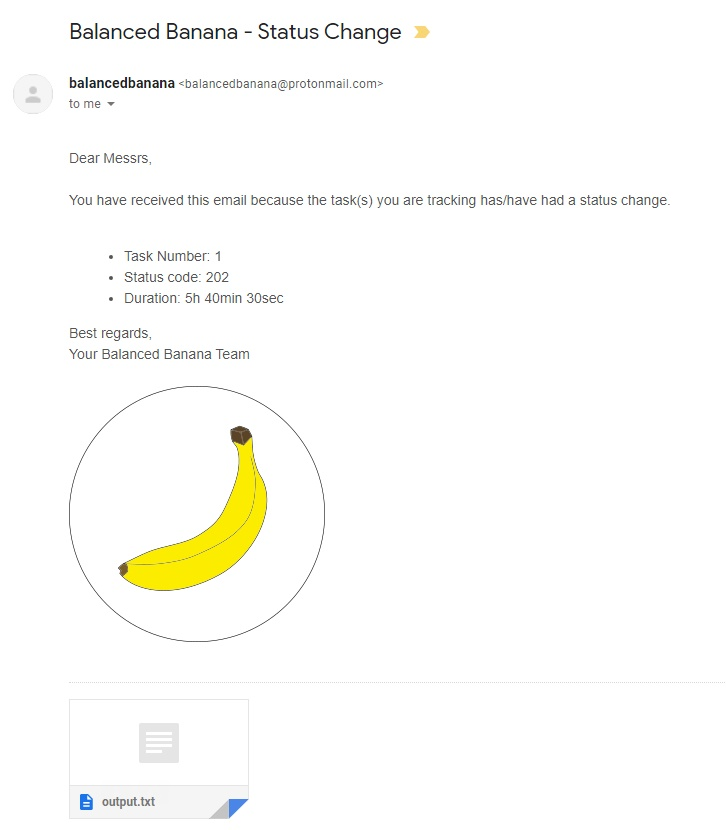
\includegraphics[width=\paperwidth]{beispiel_email.png}}
\end{center}
\clearpage

\section{Qualitätszielbestimmungen}
% Tabelle ... schafeln .. was ist ihm wichtig

\begin{comment}

%Format eines Testfalls:
\begin{minipage}[t]{\linewidth}
\item[FA00] \textbf{<Titel>}
\subitem \textbf{Erklärung} <Was soll getestet werden>
\subitem \textbf{Ablauf} <Vorbedingung/Startzustand>
<Eine Sequenz von Aktionen und Zwischenzuständen>
<Nachbedingung/Endzustand>
<Alle Zustände können auch wegfallen>
\end{minipage}
\pagebreak
%Ende der Vorlage

\end{comment}

\clearpage
\section{Testfälle/Testszenarien}
\subsection{Grundlegende Testfälle}

\begin{itemize}
\item[T01] \textbf{Verbinden des Clients mit dem Server (FA1, FA2, FA3)}
\subitem \textbf{Erklärung} Ziel ist zu testen, ob sich der Client beim Programstart automatisch mit dem Server verbinden kann.
\subitem \textbf{Ablauf} Ausgegangen wird von einem bereits laufenden System, das mindestens aus dem Server und einem Arbeiter besteht.
Der Nutzer versucht eine Aufgabe zu erstellen.
Wenn das System funktioniert, bekommt er die Job-Id seiner Aufgabe zurück.
Bekommt er die Fehlermeldung
\begin{mycode}
Error: Can not find server
\end{mycode}
so konnte keine Verbindung zum Server hergestellt werden. Erhält er die Fehlermelung
\begin{mycode}
Error: Could not authenticate to the server
\end{mycode}
so konnte der Nutzer sich nicht gegenüber dem Server authentisieren. Erhält er eine andere Fehlermeldung, so konnte die Aufgabe nicht gestartet werden.

\item[T02] \textbf{Speichern von Parametern in dem \gls{Configfile} (FA41 FA42)}
\subitem \textbf{Erklärung} Ziel ist zu testen, ob im \gls{Configfile} angegebene Einstellungen beim Erstellen von Aufgaben berücksichtigt werden.
\subitem \textbf{Ablauf} Ausgegangen wird von einem bereits funktionierenden System, in dem Aufgaben an Arbeiter verteilt werden können.
Der Nutzer trägt in das \gls{Configfile} eine maximale Speichernutzung von einem Kilobyte ein und erstellt eine Aufgabe, die 2 Kilobyte benötigt.
Bekommt er eine Benachrichtigung, dass das Programm abgestürzt ist, weil der Speicher vollgelaufen ist, wird das \gls{Configfile} korrekt mit einbezogen.

\item[T03] \textbf{Festlegen von Prioritäten (FA 43)}
\subitem \textbf{Erklärung} Ziel ist zu testen, ob Aufgaben mit einer höheren \gls{Prioritaet} bevorzugt werden.
\subitem \textbf{Ablauf} Ausgegangen wird von einem bereits funktionierenden System mit genau einem Arbeiter, in dem Aufgaben verteilt und bearbeitet werden können.
Der Nutzer startet eine Aufgabe die einige Zeit benötigt. Während der Bearbeitung gibt er eine Aufgabe mit einer niedrigen \gls{Prioritaet} auf gefolgt von derselben Aufgabe mit einer hohen Priorität.
Sind alle drei Aufgaben bearbeitet, startet er wieder eine Aufgabe, die einige Zeit benötigt. Danach erstellt er eine Aufgabe mit einer hohen \gls{Prioritaet} und danach dieselbe Aufgabe mit niedriger Priorität.
Wenn das System korrekt funktioniert, werden in beiden Fällen die Aufgaben mit hoher \gls{Prioritaet} zuerst bearbeitet.

\item[T04] \textbf{Festlegen von minimal und maximal bereitgestellten CPU-Kernen (FA44)}
\subitem \textbf{Erklärung} Ziel ist zu testen, ob der Nutzer festlegen kann wie viele Kerne einer Aufgabe zur Verfügung gestellt werden sollen.
\subitem \textbf{Ablauf} Da jede Aufgabe in einem eigenen Container ausgeführt wird, reicht es aus eine Aufgabe zu starten, die die Anzahl der CPU-Kerne der virtuellen Umgebung ausgibt und diese Aufgabe mit verschiedenen Werten aufgibt.

\item[T05] \textbf{Festlegen von maximal nutzbarem RAM (FA45)}
\subitem \textbf{Erklärung} Ziel ist zu testen, ob der Nutzer festlegen kann wie viel Hauptspeicher seiner Anwendung zur Verfügung gestellt werden soll.
\subitem \textbf{Ablauf} Ausgegangen wird von einem funktionierenden System, in dem der Nutzer Aufgaben erstellen kann, die bearbeitet werden.
Der Nutzer startet eine Aufgabe, die mindestens 2 Kilobyte Speicher anfordert und stellt der Aufgabe einen maximalen Hauptspeicher von einem Kilobyte zur Verfügung.
Bekommt er eine Nachricht, dass der Speicher vollgeöaufen ist und die Aufgabe deshalb abgebrochen werden musste, funktioniert das System.

\item[T06] \textbf{Festlegen des Betriebssystems/des zu verwendenden Containers (FA46)}
\subitem \textbf{Erklärung} Ziel ist zu testen, ob der Nutzer verschiedene Container angeben kann, die für die Bearbeitung seiner Aufgabe verwendet werden sollen.
\subitem \textbf{Ablauf} Ausgegangen wird von einem funktionierenden System, das Aufgaben entgegennehmen und bearbeiten kann.
Der Nutzer erstellt einen Container auf dem ein Program X installiert ist und einen identischen Container, auf dem aber X nicht installiert ist.
Dann startet er eine Aufgabe, die das Programm aufrufen soll mit den unterschiedlichen Containern. Wenn das System funktioniert, dann wird genau eine Aufgabe mit einem Fehler beenden und die andere wird korrekt ausgeführt werden.

\item[T07] \textbf{Festlegen der Pausierbareit einer Aufgabe (FA47)}
\subitem \textbf{Erklärung} Ziel ist zu testen, ob der Nutzer festlegen kann, ob seine Aufgabe pausiert werden darf und ob das System dies berücksichtigt.
\subitem \textbf{Ablauf} Ausgegangen wird von einem funktionierenden System, das Aufgaben entgegennimmt und bearbeitet.
Der Nutzer erstellt eine Aufgabe und gint an, dass diese pausierbar sein soll. Während die Aufgabe bearbeitet wird, versucht er über seine Konsole die Aufgabe zu pausieren.
Funktioniert das, erstellt er dieselbe Aufgabe erneut, aber lässt sie nicht pausierbar sein. Er versucht erneut die AUfgabe zu pausieren.
Falls das System korrekt funktioniert, lässt sich diese Aufgabe nicht pausieren und der Nutzer bekommt eine Fehlermeldung angezeigt.

\item[T08] \textbf{Abfragen eines Aufgabenstatus (FA 5 FA51)}
\subitem \textbf{Erklärung} Ziel ist zu testen, ob der Nutzer den korrekten Status seiner Aufgaben abfragen kann.
\subitem \textbf{Ablauf} Ausgegangen wird von einem funktionierenden System mit genau einem Arbeiter, das Aufgaben entegennehmen und verarbeiten kann.
Der Nutzer erstellt eine Aufgabe, die den ganzen Worker auslastet und ruft ihren Status ab. Er sollte als Rückmeldung "processing" erhalten. Bevor die erste Aufgabe abgearbeitet ist, erstellt er eine weitere.
Von dieser Aufgabe ruft er ebenfalls den Status ab. Funktioniert das System korrekt, bekommt der Nutzer "scheduled" als Antwrt zurück.
Danach ruft der Nutzer den Status einer nicht vorhandenen Aufgabe ab. Jetzt sollte er eine Fehlermeldung zurück bekommen.
Als nächstes wartet er auf den Abschluss seiner ersten Aufgabe und ruft erneut ihren Status ab. Nun sollte er "finished" als Antwort erhalten.
Zuletzt ruft er noch einmal den Status der zweiten Aufgabe ab, dieser solle jetzt "processing" sein.

\item[T09] \textbf{Benachrichtigung bei Abschluss einer Aufgabe (FA 6)}
\subitem \textbf{Erklärung} Ziel ist zu testen, ob der Nutzer nach Beendigung einer Aufgabe vom System benachrichtigt wird.
\subitem \textbf{Ablauf} Ausgegangen word von einem funktionierenden System, das in der Lage ist Aufgaben anzunehmen und zu verarbeiten.
Der Nutzer erstellt zunächst eine Aufgabe, die nur aus dem Aufruf
\begin{mycode}
sleep 10
\end{mycode}
besteht und gibt seine Mail-Adresse an, entweder als Parameter in der Konsole oder als Eintrag im \gls{Configfile}.
Er wartet 2 Minuten und aktualisiert ab und zu seine Mailbox. Bis dahin ist die Aufgabe abgearbeitet und der Mailserver sollte genug Zeit bekommen haben, die Mail zuzustellen.
Funktioniert das System, so hat er eine Bestätigungsmail vom System erhalten.

\item[T10] \textbf{Erstellen von Sicherungen (FA 7)}
\subitem \textbf{Erklärung} Ziel ist zu testen, ob das System regelmäßige Sicherungen seiner Aufgaben anlegt.
\subitem \textbf{Ablauf} Ausgegangen wird von einem funktionierenden System, das in der Lage ist Aufgaben entgegen zu nehmen und zu verarbeiten.
Der Administrator setzt zuerst das Backup-Intervall des Servers auf eine Minute.
Dann startet der Nutzer eine Aufgabe, die nur aus dem Aufruf
\begin{mycode}
sleep 130
\end{mycode}
besteht. Nachdem die Aufgabe abgearbeitet ist, schaut der Administrator nach, ob im Dateisystem Sicherungen der Aufgabe liegen.
Falls das System korrekt funktioniert, findet er genau zwei dieser Sicherungen vor.
Am Schluss setzt der Administrator das Backup-Intervall wieder zurück.

\item[T11] \textbf{Anforderung der Standard-Ausgabe (FA 8)}
\subitem \textbf{Erklärung} Ziel ist zu testen, ob der Nutzer in der Lage ist sich die korrekte Standardausgabe seiner Aufgabe anzusehen
\subitem \textbf{Ablauf} Ausgegangen wird von einem funktionierenden System mit genau einem Arbeiter, das in der Lage ist Aufgaben entgegen zu nehmen und zu verarbeiten.
Der Nutzer führt eine kleine Aufgabe lokal bei sich aus und gibt sie auch an das System weiter. Er sorgt dafür, dass diese Aufgabe alle Resourcen des Arbeiters für sich beansprucht.
Dann fragt der die Ausgabe der Aufgabe ab und vergleicht sie mit seiner lokalen Ausgabe.
Bevor die Aufgabe abgeschlossen ist, erstellt er noch eine weitere Aufgabe und ruft direkt die Ausgabe ab.
Wenn das System funktioniert, bekommt er eine Fehlermeldung zurück, die ihn darauf hinweist, dass die Aufgabe noch nicht begonnen ist, sondern noch in der Warteschlange hängt.
Dann versucht der Nutzer die Ausgabe einer Aufgabe anzufordern, die es nicht gibt. Auch hier sollte er eine Fehlermeldung erhalten.
Als letztes wartet er, bis seine erste Aufgabe abgeschlossen ist und fragt dann die Ausgabe der zweiten Aufgabe ab. Jetzt sollte er keine Fehlermeldung mehr erhalten.

\end{itemize}

\subsection{Erweiterte Testfälle}

\begin{itemize}

\item[T12] \textbf{Abbrechen von zu langen Aufgaben (OFA2)}
\subitem \textbf{Erklärung} Ziel ist zu testen, ob der Server in der Lage ist Aufgaben, die zu viel Zeit benötigen, abzubrechen.
\subitem \textbf{Ablauf} Ausgegangen wird von einem funktionierenden System, das in der Lage ist Aufgaben entgegenzunehmen und zu verarbeiten und den Auftraggeber nach Abschluss einer Aufgabe zu benachrichtigen.
Der Administrator setzt die maximale Bearbeitungszeit für Aufgaben auf 1 Minute.
Danach erstellt der Benutzer eine Aufgabe, die 30 Sekunden für die Bearbeitung benötigt und eine Aufgabe, die 2 Minuten benötigt.
Wenn das System korrekt funktioniert, bekommt er eine Benachrichtigung, dass seine erste Aufgabe abgeschlossen wurde,
und eine zweite Nachricht, die ihn darauf hinweist, dass seine Aufgabe die zulässige Zeit überschritten hat.
Der Administrator setzt zuletzt die maximale Bearbeitungszeit zurück.

\item[T13] \textbf{Manuelles Stoppen von Aufgaben (OFA3)}
\subitem \textbf{Erklärung} Ziel ist zu testen, ob der Nutzer in der Lage ist seine Aufgaben selbst abzubrechen.
\subitem \textbf{Ablauf} Ausgegangen wird von einem funktionierenden System, das in der Lage ist Aufgaben entegenzunehmen, zu verarbeiten und den Status von Aufgaben zurückzugeben.
Der Nutzer gibt eine Aufgabe auf, die einige Zeit zur Abarbeitung benötigt. Als nächstes gibt er eine zweite Aufgabe auf, die sich nicht selbst beenden kann.
Dann versucht er diese zweite Aufgabe manuell zu beenden. Wenn das System funktioniert, bekommt der Nutzer, wenn er den Status der Aufgabe anfragt, "cancelled" zurück.
Außerdem sollte der Status der ersten Aufgabe weiterhin "processing" sein.

\item[T14] \textbf{Manuelle Sicherung von Aufgaben (OFA4)}
\subitem \textbf{Erklärung} Ziel ist zu testen, ob der Nutzer seine Aufgaben manuell sichern kann.
\subitem \textbf{Ablauf} Ausgegangen wird von einem System, das in der Lage ist Aufgaben entgegenzunehmen und zu bearbeiten.
Der Nutzer gibt eine Aufgabe auf, die einige Zeit zur Abarbeitung benötigt.
Als nächstes versucht er seine Aufgabe zu sichern.
Dann sieht der Administrator nach, ob im Dateisystem eine Sicherung der Aufgabe vorhanden ist.

\end{itemize}

\clearpage
\printnoidxglossaries

\end{document}
